
\item A solid body rotates about a stationary axis according to the law $\varphi = at - bt^3$, where $a = 6.0 \text{ rad/s}^2$ and $b = 2.0 \text{ rad/s}^3$. Find:
    \begin{center}
        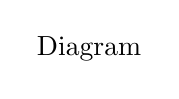
\begin{tikzpicture}
            \node at (0, 0) {Diagram}; % Replace this with the actual diagram code
        \end{tikzpicture}
    \end{center}
    \begin{enumerate}
        \item the mean values of the angular velocity and angular acceleration averaged over the time interval between $t = 0$ and the complete stop;
        \item the angular acceleration at the moment when the body stops.
    \end{enumerate}

\begin{solution}
    \begin{center}
        \begin{tikzpicture}
            \pic at (0, 0) {frame=3cm};
        \end{tikzpicture}
    \end{center}
    
    \begin{align*}
        \intertext{Let us take the rotation axis as $z$-axis whose positive direction is associated with the positive direction of the coordinate $\varphi$, the rotation angle, in accordance with the right-hand screw rule.}
        \intertext{(a) Differentiating $\varphi(t)$ with respect to time twice, we get}
        \dfrac{d\varphi}{dt} &= a - 3bt^2 = \omega_z \tag{1}\\
        \dfrac{d^2 \varphi}{dt^2} &= \dfrac{d\omega_z}{dt} = \beta_z = -6bt \tag{2}\\
        \intertext{From Eq. (1) the solid body comes to stop at}
        \Delta t = t &= \sqrt{\dfrac{a}{3b}}\\
        \intertext{The angular velocity $\omega = a - 3bt^2$, for $0 \leq t \leq \sqrt{a/3b}$}
        \left<\omega\right> &= \dfrac{\int\limits_0^{\sqrt{a/3b}} \omega dt}{\int\limits_0^{\sqrt{a/3b}} dt} = \dfrac{\int\limits_0^{\sqrt{a/3b}} (a - 3bt^2) dt}{\int\limits_0^{\sqrt{a/3b}} dt}\\
        &= \dfrac{\left[at - bt^3\right]_0^{\sqrt{a/3b}}}{\sqrt{a/3b}} = \dfrac{2a/3}{1} = 4\ \text{rad/s}
        \intertext{Similarly, $\beta = \lvert \beta_z \rvert = 6bt$ for all values of $t$.}
        \left<\beta\right> &= \dfrac{\int\limits_0^{\sqrt{a/3b}} \beta dt}{\int\limits_0^{\sqrt{a/3b}} dt} = \dfrac{\int\limits_0^{\sqrt{a/3b}} 6bt\ dt}{\sqrt{a/3b}} = \sqrt{3ab} = 6\ \text{rad/s}^2
        \intertext{(b) From Eq. (2),}
        \beta_z &= -6bt\\
        \left(\beta_z\right)_{t=\sqrt{a/3b}} &= -6b\sqrt{\dfrac{a}{3b}} = -2\sqrt{3ab}\\
        \intertext{Hence,}
        \beta &= \left\lvert \left(\beta_z\right)_{t=\sqrt{a/3b}} \right\lvert = 2\sqrt{3ab} = 12\ \text{rad/s}^2
    \end{align*}
\end{solution}